% Options for packages loaded elsewhere
\PassOptionsToPackage{unicode}{hyperref}
\PassOptionsToPackage{hyphens}{url}
\PassOptionsToPackage{dvipsnames,svgnames,x11names}{xcolor}
%
\documentclass[
  12pt]{article}

\usepackage{amsmath,amssymb}
\usepackage{iftex}
\ifPDFTeX
  \usepackage[T1]{fontenc}
  \usepackage[utf8]{inputenc}
  \usepackage{textcomp} % provide euro and other symbols
\else % if luatex or xetex
  \usepackage{unicode-math}
  \defaultfontfeatures{Scale=MatchLowercase}
  \defaultfontfeatures[\rmfamily]{Ligatures=TeX,Scale=1}
\fi
\usepackage{lmodern}
\ifPDFTeX\else  
    % xetex/luatex font selection
\fi
% Use upquote if available, for straight quotes in verbatim environments
\IfFileExists{upquote.sty}{\usepackage{upquote}}{}
\IfFileExists{microtype.sty}{% use microtype if available
  \usepackage[]{microtype}
  \UseMicrotypeSet[protrusion]{basicmath} % disable protrusion for tt fonts
}{}
\makeatletter
\@ifundefined{KOMAClassName}{% if non-KOMA class
  \IfFileExists{parskip.sty}{%
    \usepackage{parskip}
  }{% else
    \setlength{\parindent}{0pt}
    \setlength{\parskip}{6pt plus 2pt minus 1pt}}
}{% if KOMA class
  \KOMAoptions{parskip=half}}
\makeatother
\usepackage{xcolor}
\setlength{\emergencystretch}{3em} % prevent overfull lines
\setcounter{secnumdepth}{5}
% Make \paragraph and \subparagraph free-standing
\ifx\paragraph\undefined\else
  \let\oldparagraph\paragraph
  \renewcommand{\paragraph}[1]{\oldparagraph{#1}\mbox{}}
\fi
\ifx\subparagraph\undefined\else
  \let\oldsubparagraph\subparagraph
  \renewcommand{\subparagraph}[1]{\oldsubparagraph{#1}\mbox{}}
\fi


\providecommand{\tightlist}{%
  \setlength{\itemsep}{0pt}\setlength{\parskip}{0pt}}\usepackage{longtable,booktabs,array}
\usepackage{calc} % for calculating minipage widths
% Correct order of tables after \paragraph or \subparagraph
\usepackage{etoolbox}
\makeatletter
\patchcmd\longtable{\par}{\if@noskipsec\mbox{}\fi\par}{}{}
\makeatother
% Allow footnotes in longtable head/foot
\IfFileExists{footnotehyper.sty}{\usepackage{footnotehyper}}{\usepackage{footnote}}
\makesavenoteenv{longtable}
\usepackage{graphicx}
\makeatletter
\def\maxwidth{\ifdim\Gin@nat@width>\linewidth\linewidth\else\Gin@nat@width\fi}
\def\maxheight{\ifdim\Gin@nat@height>\textheight\textheight\else\Gin@nat@height\fi}
\makeatother
% Scale images if necessary, so that they will not overflow the page
% margins by default, and it is still possible to overwrite the defaults
% using explicit options in \includegraphics[width, height, ...]{}
\setkeys{Gin}{width=\maxwidth,height=\maxheight,keepaspectratio}
% Set default figure placement to htbp
\makeatletter
\def\fps@figure{htbp}
\makeatother

\addtolength{\oddsidemargin}{-.5in}%
\addtolength{\evensidemargin}{-1in}%
\addtolength{\textwidth}{1in}%
\addtolength{\textheight}{1.7in}%
\addtolength{\topmargin}{-1in}%
\makeatletter
\@ifpackageloaded{caption}{}{\usepackage{caption}}
\AtBeginDocument{%
\ifdefined\contentsname
  \renewcommand*\contentsname{Table of contents}
\else
  \newcommand\contentsname{Table of contents}
\fi
\ifdefined\listfigurename
  \renewcommand*\listfigurename{List of Figures}
\else
  \newcommand\listfigurename{List of Figures}
\fi
\ifdefined\listtablename
  \renewcommand*\listtablename{List of Tables}
\else
  \newcommand\listtablename{List of Tables}
\fi
\ifdefined\figurename
  \renewcommand*\figurename{Figure}
\else
  \newcommand\figurename{Figure}
\fi
\ifdefined\tablename
  \renewcommand*\tablename{Table}
\else
  \newcommand\tablename{Table}
\fi
}
\@ifpackageloaded{float}{}{\usepackage{float}}
\floatstyle{ruled}
\@ifundefined{c@chapter}{\newfloat{codelisting}{h}{lop}}{\newfloat{codelisting}{h}{lop}[chapter]}
\floatname{codelisting}{Listing}
\newcommand*\listoflistings{\listof{codelisting}{List of Listings}}
\makeatother
\makeatletter
\makeatother
\makeatletter
\@ifpackageloaded{caption}{}{\usepackage{caption}}
\@ifpackageloaded{subcaption}{}{\usepackage{subcaption}}
\makeatother
\ifLuaTeX
  \usepackage{selnolig}  % disable illegal ligatures
\fi
\usepackage[]{natbib}
\bibliographystyle{agsm}
\usepackage{bookmark}

\IfFileExists{xurl.sty}{\usepackage{xurl}}{} % add URL line breaks if available
\urlstyle{same} % disable monospaced font for URLs
\hypersetup{
  pdftitle={Are you normal? A new projection pursuit index to assess a sample against a multivariate null distribution},
  pdfauthor={Annalisa Calvi, Ursula Laa, Dianne Cook},
  colorlinks=true,
  linkcolor={blue},
  filecolor={Maroon},
  citecolor={Blue},
  urlcolor={Blue},
  pdfcreator={LaTeX via pandoc}}


\begin{document}


\def\spacingset#1{\renewcommand{\baselinestretch}%
{#1}\small\normalsize} \spacingset{1}


%%%%%%%%%%%%%%%%%%%%%%%%%%%%%%%%%%%%%%%%%%%%%%%%%%%%%%%%%%%%%%%%%%%%%%%%%%%%%%

\title{\bf Are you normal? A new projection pursuit index to assess a
sample against a multivariate null distribution}
\author{
Annalisa Calvi, Ursula Laa, Dianne Cook\\
}
\maketitle

\bigskip
\bigskip
\begin{abstract}

\end{abstract}


\newpage
\spacingset{1.9} % DON'T change the spacing!

\section{Introduction}\label{introduction}

Linear projections are useful in many aspects of statistical analysis of
multivariate data, and especially useful for visualising the data. A
linear projection provides a dimension reduction while maintaining
interpretability. For example, a biplot (REF) shows the structure
creating the maximum variance in the data, and also visualizing the
projection matrix to learn which variables contribute to it. We might
find clusters of outliers that were hiding in high dimensions.

More generally, projection pursuit (REF) defines a quantitative
criterion for the interestingness of a projection (a projection pursuit
index), and searches the space of possible projections for the most
interesting one to display. We can also define sequences of interpolated
linear projections to better understand a multivariate distribution.
Animating a randomly selected interpolated sequence of linear
projections is called a grand tour (REF). The combination of these two
approaches would then use a projection pursuit index to select
interesting projections, but display them via an interpolated path to
provide context. This is called a guided tour (REF).

The question is whether we can use these techniques to assess new data
samples in the context of an established normal, such as a specific
multivariate normal distribution. In physics, the normal distribution
may describe experimental results, or a global fit for a selected model,
and we might want to compare to a set of other models. In medical
applications, the normal distribution might summarize historic data of a
healthy population and we compare it to samples from new patients. In
outlier detection we might use robust measures to define the normal
distribution and look for anomalies.

This paper describes a new projection pursuit index which is optimized
by projections where a new sample is most distant from the existing
normal distribution. It is organised as follows.
Section~\ref{sec-background} provides more context for the methods and
visualisation. Section~\ref{sec-anomaly-index} provides the details of
the new index, and example use is illustrated in
Section~\ref{sec-examples}.

\section{Background}\label{sec-background}

To compare a new sample with an existing norm, like a multivariate
normal distribution, in higher than two dimensions, we have typically
used two samples of points. The norm is represented by points on the
surface of a \(p\)-dimensional ellipse, corresponding to a confidence
level. A sample of points uniformly distributed on a \(p\)-dimensional
sphere is generated by

\begin{enumerate}
\def\labelenumi{\arabic{enumi}.}
\tightlist
\item
  Simulating a sample of observations from \(N_p(\mu, \Sigma)\).
\item
  Transforming each observation to have unit distance from the mean.
\end{enumerate}

\begin{figure}[H]

{\centering 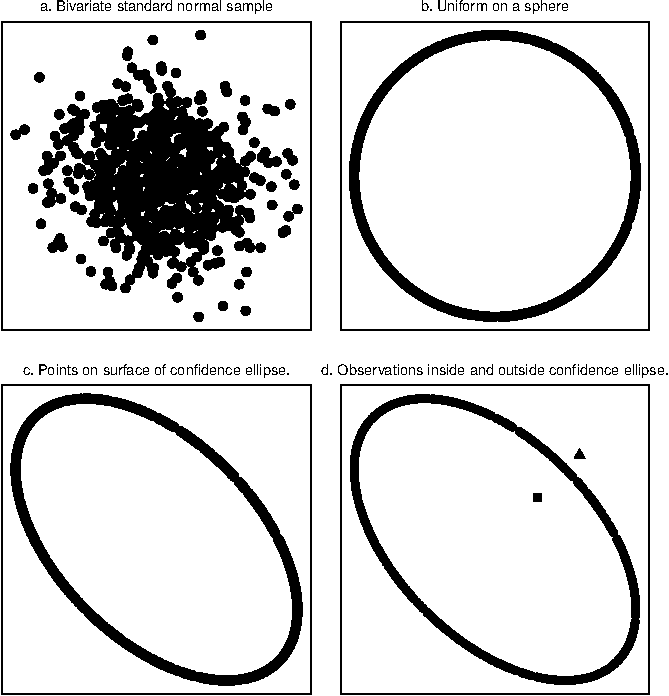
\includegraphics[width=1\textwidth,height=\textheight]{paper_files/figure-pdf/unnamed-chunk-4-1.pdf}

}

\caption{Simulating a uniform sample on a sphere involves sampling from
a multivariate normal (a) and transforming each observation to have
length equal to 1. A confidence ellipse is generated by transforming the
sphere relative to a specified variance-covariance matrix (c), and new
observations can be visually assessed to be inside or outside by
plotting with the ellipse (d).}

\end{figure}%

\section{Anomaly index}\label{sec-anomaly-index}

\section{Examples}\label{sec-examples}



\end{document}
